%%%%%%%%%%%%%%%%%%%%%%%%%%%%%%%%%%%%%%%%%%%
%%% DOCUMENT PREAMBLE %%%
\documentclass[12pt]{report}
\usepackage[english]{babel}
%\usepackage{natbib}
\usepackage{url}
\usepackage[utf8x]{inputenc}
\usepackage{amsmath}
\usepackage{graphicx}
\graphicspath{{images/}}
\usepackage{parskip}
\usepackage{fancyhdr}
\usepackage{vmargin}
\usepackage[T1]{fontenc} % Use 8-bit encoding that has 256 glyphs
\usepackage{booktabs} % for nice lines in tables
\setmarginsrb{3 cm}{2.5 cm}{3 cm}{2.5 cm}{1 cm}{1.5 cm}{1 cm}{1.5 cm}

\title{Applying Reinforcement Learning to Bomberman}								
% Title
\author{Hein-Erik Schnell, Karl Thyssen}						
% Author
\date{\today}
% Date

\makeatletter
\let\thetitle\@title
\let\theauthor\@author
\let\thedate\@date
\makeatother

\pagestyle{fancy}
\fancyhf{}
\rhead{\theauthor}
\lhead{\thetitle}
\cfoot{\thepage}

% displays code within text
\newcommand{\code}[1]{{\fontfamily{pcr}\selectfont #1}}
\newcommand{\state}[1]{$\left\lbrace #1 \right\rbrace$}
%%%%%%%%%%%%%%%%%%%%%%%%%%%%%%%%%%%%%%%%%%%%
\begin{document}

%%%%%%%%%%%%%%%%%%%%%%%%%%%%%%%%%%%%%%%%%%%%%%%%%%%%%%%%%%%%%%%%%%%%%%%%%%%%%%%%%%%%%%%%%

\begin{titlepage}
	\centering
    \vspace*{0.5 cm}
    
\includegraphics[scale = 0.075]{uni_hd_logo.jpg}\\[1.0 cm]	% University Logo
\begin{center}    \textsc{\Large   Fundamentals of Machine Learning}\\[2.0 cm]	\end{center}% University Name
	\textsc{\Large Final Project  }\\[0.5 cm]				% Course Code
	\rule{\linewidth}{0.2 mm} \\[0.4 cm]
	{ \huge \bfseries \thetitle}\\
	\rule{\linewidth}{0.2 mm} \\[1.5 cm]
	
	\begin{minipage}{0.4\textwidth}
		\begin{flushleft} \large
		%	\emph{Submitted To:}\\
		%	Name\\
          % Affiliation\\
           %contact info\\
			\end{flushleft}
			\end{minipage}~
			\begin{minipage}{0.4\textwidth}
            
			\begin{flushright} \large
			\emph{Submitted By :} \\
			Hein-Erik Schnell\\
			Karl Thyssen  
		\end{flushright}
           
	\end{minipage}\\[2 cm]
	
	%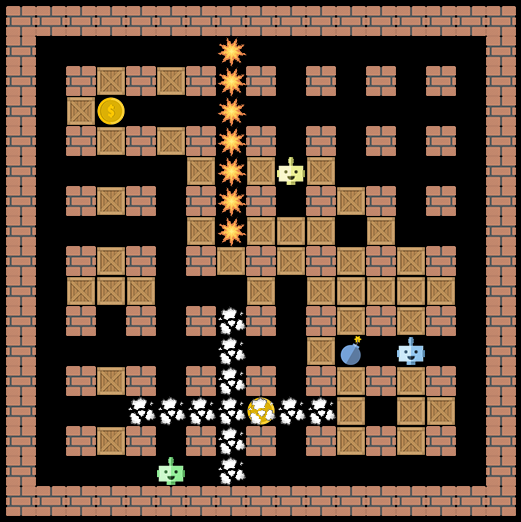
\includegraphics[scale = 0.3]{Bomberman_title.png}
    
    
    
    
	
\end{titlepage}

%%%%%%%%%%%%%%%%%%%%%%%%%%%%%%%%%%%%%%%%%%%%%%%%%%%%%%%%%%%%%%%%%%%%%%%%%%%%%%%%%%%%%%%%%

\tableofcontents
\pagebreak

%%%%%%%%%%%%%%%%%%%%%%%%%%%%%%%%%%%%%%%%%%%%%%%%%%%%%%%%%%%%%%%%%%%%%%%%%%%%%%%%%%%%%%%%%
\renewcommand{\thesection}{\arabic{section}}
\section{Heins thoughts}
Tasks to be done are:
	\begin{itemize}
		\item Find a suitable \textit{state representation} to be then passed to an estimator to estimate the expected reward for each of the possible actions
		\item Find a suitable rewards in order to communicate the goals of the game to the agent
		\item Find a suitable model which estimates the expected reward for each possible action at the current state of the game.
	\end{itemize}

\subsection{State representation}
My proposal is a 2D numpy array. Each row (first index) represents a single state. Each column represents a feature. All available information is stored within each agent in the dictionary \code{self.game\_state}. What features do we store?
	\begin{itemize}
		\item For each cell:
		\begin{itemize}
			\item \textbf{Crate, wall, free \state{1,-1,0}}: The same representation is provided by \code{self.game\_state}. Only it has to be reshaped into a 1D-array. 
			\item \textbf{Cell contains agent \state{0,1}}
			\item \textbf{Cell contains opponent \state{0,1}}: This and the point above need to be stored seperately because it is possible for agent and opponent to occupy the same cell. It would just be impossible to distinguish whether a cell is occupied by just one or more opponents. But this should be a negligible issue. 
			\item \textbf{Cell contains coin \state{0,1}}
			\item \textbf{Explosion on cell}: Provided as 2D-numpy array by \code{self.game\_state}.
			\item \textbf{Danger level \state{0,\dots,4}}: How many time steps until an explosion will hit the cell.
		\end{itemize}
		\item Just once at the end of the array:
		\begin{itemize}
			\item \textbf{Current step number \state{1,\dots,400}}
			\item \textbf{Bomb action possible \state{0,1}}
			\item \textbf{Danger level:} This is a danger level for the agent. It is not necessary but provides a clearer measure of whether the agent is actually in danger. I propose to calculate this by multiplicating the danger level of each cell with the \textit{Cell contains agent} entry of each cell and then take the maximum of all the results. This way we will only get a non-zero value if the agent is on a cell with a danger level $>0$.
			\item \textbf{Reward already received in this episode}
			\item \textbf{Reward received at the end of the episode}: This one has to be added subsequently at the end of the episode to each ocurred state.
			\item \textbf{Reward gained after this state occurred:} This one is the difference of the two above. This should be our \textit{target} which we aim to maximize.
		\end{itemize}
	\end{itemize}
This gives us $6$ entries for each cell and $6$ entries at the end of the array. There are $17\times17$ cells in the arena. However, the cells located at the rim are always \textit{walls}. These do not need to be stored. What remains is a $15\times15$ grid. I am not sure whether we want to store cells with \textit{walls} at all, because these are always the same. They should add nothing to the state of the game.\\
Therefore we have $15\times15=225$ entries ($15\times15-7\times7=176$ if we don't store walls) plus $6$ at the end of the array for each state (time step). Storing these total $231$($182$) entries in a numpy array might produce big amounts of data. We should consider specifying the data type explicitly. However, the numpy documentation states that the data type is chosen as the minimum type required to hold the objects in the sequence.

\subsection{Rewards}
The most rewarded actions should be those which will win us the game. Those are collecting coins (1 point) and killing opponents (5 points). Therefore, I propose the same scaling between those two when rewarding them. \\
Subgoals which we consider helpful for winning should be rewarded too, but only with few points. It should be almost impossible to substitute the \textit{winning actions} (coins and killing) with \textit{helpful actions} (destroying crates). \\
I also propose a penalty of $-1$ for every action so that the agent learns to act as efficiently as possible. \\
Dying should be (beware! wordplay:) gravely punished. 
\begin{figure}[h]
	\centering
	\begin{tabular}{c|c}
		Action & Reward\\
		\toprule
		Collect coin & 100\\
		Kill opponent & 500\\
		Destroy crate & 1-2 per crate\\
		Perform action & -1\\
		Die & -500fd
	\end{tabular}
\end{figure}

\subsection{Estimator} 
I don't know much about neural networks which is why I spent most of my thoughts on how to implement this with the models we used in the exercises. Plus, I like the idea of the challenge to come up with an agent which doesn't use a neural network. \\
Since we want to estimate the expected reward of performing an action at in a given state, we need a regressor. This regressor needs to be highly flexible in order to cope with the variety of states. I guess the most flexible regressor we used would be a \textit{Random Forest Regressor}. On the one hand, this one would need tons of learning data but on the other hand, which proper regressor doesn't?\\
This means, we would plug the data of the states and the received rewards into the model and get an estimate of what reward we could expect for what action. Since we need to distinguish between the six possible actions, we need six Random Forests. One for each action. Each forest trained only with the states after which the respective action was performed. 

\subsection{Learning algorithm}
I propose to use the Max-Boltzmann method as described in \cite{paper} or something similar. It is mostly a $\epsilon$-greedy algorithm. But when it decides to explore, it doesn't choose randomly among the remaining actions but assigns probabilities corresponding to the value (expected reward) of the remaining action. This way, exploration is not just random but more targeted.
\subsection{Necessary functions}
Some functions that need to be implemented in order to prepare everything:
\begin{itemize}
	\item Calculate danger levels of each cell
	\item Insert \textit{coins} into state array
	\item Insert \textit{opponents} into state array
	\item Insert \textit{self} into state array
\end{itemize}
We need to decide what structure the \textit{state vector} should have. There are two ways:
\begin{enumerate}
	\item All features of a concerning cell (coin, opponent, self, danger level,...) subsequently. The all features of the next cell and so on \dots
	\item All data of one feature (e.g. coin) for all cells, then all data of the next feature for all cells and so on \dots
\end{enumerate}
In both cases, the functions that insert the values into the array should make use of the slicing possibilities of numpy arrays (e.g. \code{x[starting point:end point:stepsize]}). In the first case, only every sixth entry represents the same feature. In the second case, the first hundred entries represent only one feature for different cells.


%%%%%%%%%%%%%%%%%%%%%%%%%%%%%%%%%%%%%%%%%%%%%%%%%%%%%%%%%%%%%%%%%%%%%%%%%%%%%%%%%%%%%%%%%
\begin{thebibliography}{111}
   

%if the "underfill \hbox" warning bothers you uncomment the following line
%\raggedright


\bibitem{RL_intro}
Richard S. Sutton, Andrew G. Barto (2018)\\
\textit{Reinforcement Learning: An Introduction}\\
Available at: http://incompleteideas.net/book/bookdraft2018jan1.pdf

\bibitem{paper}
Joseph Groot Kormelink, Madalina M. Drugan and Marco A. Wiering (ICAART 2018)\\
\textit{Exploration Methods for Connectionist Q-Learning in Bomberman}\\
Available at: https://bit.ly/2GReSxQ
\end{thebibliography}
\end{document}

%This template was created by Roza Aceska.